
%(BEGIN_QUESTION)
% Copyright 2012, Tony R. Kuphaldt, released under the Creative Commons Attribution License (v 1.0)
% This means you may do almost anything with this work of mine, so long as you give me proper credit

Use the ``current triangle'' to calculate the phase shift angle ($\theta$) between total current ($I_{total}$) and resistor current ($I_R$) in this parallel resistor-inductor circuit, as well as the magnitude of total current:

$$\includegraphics[width=15.5cm]{i01942x01.eps}$$

\vskip 20pt

$\theta$ = 

\vskip 10pt

$I_{total}$ = 

\underbar{file i01942}
%(END_QUESTION)





%(BEGIN_ANSWER)

$\theta$ = 60.26$^{o}$ (negative, if you wish to represent the angle according to the standard coordinate system for phasors)

\vskip 10pt

$I_{total}$ = 16.12 A

%(END_ANSWER)





%(BEGIN_NOTES)

{\bf This question is intended for exams only and not worksheets!}.

%(END_NOTES)


